% 01_general_description.tex
\chapter{General Description and Features}
\label{ch:vol9_general_description}

\begin{objectivebox}
\begin{itemize}
    \item Identify the substrate documented in this datasheet: the natural vacuum substrate.
    \item Enumerate the load-bearing structural features (K4 Cosserat lattice, intrinsic LC oscillators, bond transmission lines, Cosserat micropolar 6 DOF/node, saturation kernel, boundary semantics).
    \item Establish the epistemic position: substrate is natural; engineering characterizes; AVE substrate-physics derives.
    \item Define the spec-table column convention used in subsequent chapters (Symbol / Typical / Min / Max / Units / Conditions / Canonical Source).
    \item Map the chapter sequence to the canonical derivation locations in Volumes I through VI.
\end{itemize}
\end{objectivebox}

\section{The Vacuum as a Component}
\label{sec:vol9_vacuum_as_component}

This datasheet documents the vacuum as a \textbf{component}, not a stage. The medium is a chiral crystal --- the \texttt{srs} net ($z=3$, $I4_132$; the ratified production carrier per D1, Grant 2026-07-03, \kbleaf{\_orchestration/index.md}) --- in which every node is a lossless LC resonator carrying six degrees of freedom: three translational (capacitive, the $\mathbf{E}$ store) and three microrotational (inductive, the $\mathbf{B}$ store), per Axiom~1 (Ch.~\ref{ch:vol9_mechanical_characteristics}). Each node additionally carries an operating point --- the saturation state $A$, a DC bias on the node's own nonlinearity (``the dynamical state of the LC tank, analogous to the DC bias on a semiconductor varactor'', Ch.~\ref{ch:vol9_saturation_characteristics}), which is \emph{not} a seventh spatial DOF. The network's characteristic impedance is $Z_0 = \sqrt{\mu_0/\varepsilon_0} \approx \qty{376.73}{\ohm}$ (\kbleaf{src/ave/core/constants.py} \texttt{Z\_0}); it is the substrate's own canonical EE primitive, and the most direct standing measurement of the medium available.

\paragraph{Transparency (the governing law).} Axiom~3 (Minimum Reflection Principle) extremizes the substrate action by minimizing the reflected fraction $|\Gamma|^2$ at every internal impedance boundary (\kbleaf{ave-kb/common/axiom-register.md}, \texttt{axiom-3}). The medium is transparent to its own radiation because it is extremal (by its own principle) against internal reflection: a matched line ($\Gamma=0$) neither reflects nor stores net bias, so light --- pure AC riding the ground state, time-averaging to zero bias --- crosses without leaving a trace. The stronger chain \emph{minimum reflection $\Rightarrow$ bond-stiffness balance ($k_s = k_a$) $\Rightarrow$ isotropy $+$ distortionless propagation} --- ``one condition, three protections'' --- is now \textbf{derived} on the ratified srs-$z=3$ net: minimizing the internal-boundary reflection $\Gamma_{\mathrm{internal}}(\rho_{\mathrm{bond}})$ over the stiffness ratio $\rho_{\mathrm{bond}} = k_a/k_s$ lands knob-free on $\rho_{\mathrm{bond}} = 1$ ($k_s = k_a$) to machine precision, where match, photon-branch isotropy, distortionlessness, and Zener-$A{=}1$ all co-locate (\kbleaf{research/2026-07-04\_parent-condition-match-forces-balance\_result.md}, verdict \textsc{[mechanism-derived]}; Axiom~3 \emph{is} the parent of the isotropy pinning). \emph{(Grade note: this is a merged research result; its propagation into a canonical KB leaf + claim-id is a gated follow-on, so the datasheet states it as a derived research verdict, not yet a canonized claim.)}

\paragraph{Absolute-maximum ratings.} Every node saturates along the Axiom~4 quarter-arc kernel $S(A) = \sqrt{1 - A^2}$. The $p=2$ (quadratic / L2-norm) exponent is \textbf{shape-derived}, not posited: the lossless bond-LC tank (Axiom~1~$+$~Axiom~3) conserves $E = \tfrac12 C V^2 + \tfrac12 \Phi^2/L$ exactly, so its dynamical phase-plane vector traces a fixed-radius circle --- the L2 invariant is forced, and \emph{only} $p=2$ satisfies it (\kbleaf{ave-kb/common/axiom-register.md} Axiom~4 provenance; \kbleaf{research/2026-07-02\_axiom4-forced\_result.md}, verdict \textsc{conditionally-forced}; the count stays 4 because the residual is itself the L2 constraint). The two thresholds on this kernel --- $V_{yield} = \sqrt{\alpha}\,V_{snap} \approx \qty{43.65}{\kV}$ (transverse-$T_2$ self-trap wall) and $V_{snap} = m_e c^2/e \approx \qty{511}{\kV}$ (longitudinal-A1 completion; \texttt{def-vyvsn1}, Grant 2026-06-30) --- are this component's absolute-maximum ratings (Ch.~\ref{ch:vol9_absolute_maximum_ratings}). Hence a datasheet.

\paragraph{Matter as a standing-wave state.} Matter is the medium's standing-wave state, not a separate substance. The electron is a knot of phase winding self-trapped at its own yield wall by total internal reflection ($\Gamma = -1$, lossless; Ch.~\ref{ch:vol9_pin_port_configuration}~\S Boundary semantics). Its \textbf{mass} is the trap's stored energy (A1 dilatation store, $E = m_e c^2$); its \textbf{spin / moment} is the circulation of that store; its \textbf{charge} is a topological integer the lattice forces --- the $\mathrm{Link}$ winding-quantum, globally \emph{neutral}, whose field strength is a calibration (the $\xi_{topo} \equiv e/\ell_{node}$ $\alpha$-echo) and whose static Coulomb field is \emph{locally unsourced}: the sourced-static-monopole route is closed at derivation grade by the four-lock no-go cascade (\texttt{clm-nogo4l}, \kbleaf{ave-kb/common/the-sourced-charge-no-go-cascade.md}). The charge label is boundary data the medium carries (a winding integer $+$ forced neutrality), not an emission from a source.

\paragraph{The honesty ledger.} The framework \emph{derives structure and imports scales} throughout: the forms are AVE's ($S(A)$ kernel shape, the A1/T2 sector split, the topological $\mathrm{Link}$ integer, the $\Gamma$-space operating points), while the scale-setting values ($\alpha$, $m_e$, $G$) are imported --- as every framework imports them (\kbleaf{ave-kb/common/form-deriving-value-importing.md}). The one pre-registered measurable divergence from the standard account: this medium's electric response saturates at \textbf{tree level} (the Axiom~4 kernel is a classical constitutive saturation, not a loop effect) --- the vacuum-birefringence falsifier. The discriminator is the field-\emph{independent} coefficient ratio of the saturation, \emph{not} an $E^4$-vs-$E^2$ exponent (both AVE and QED are $E^2$-leading in the index shift; the earlier ``$E^4$'' framing was retracted as a $\sqrt{\varepsilon}$ conflation, \texttt{clm-pp3qwf}, \kbleaf{ave-kb/vol4/falsification/index.md}; the live falsifier is the coefficient, \kbleaf{ave-kb/vol4/falsification/ch12-falsifiable-predictions/vacuum-birefringence-e4.md}).

\section{Substrate Identity}
\label{sec:vol9_substrate_identity}

What follows documents the natural vacuum substrate's measurable behavior. The substrate is the universe's own vacuum --- a 3D chiral Laves K4 Cosserat crystal with right-handed $I4_1 32$ chiral space group, 3-fold ($z=3$) chiral srs (Sunada-K4 / Laves) nearest-neighbour connectivity, and intrinsic LC oscillators at every node.\footnote{The physical \emph{connectivity} of the \texttt{srs} node is $z=3$ (three nearest-neighbour bonds; the object Axiom~1 names). The ``K4 4-port'' $A_1 \oplus T_2$ irrep decomposition used in the mode inventory (Ch.~\ref{ch:vol9_pin_port_configuration} \S K4 valence, Ch.~\ref{ch:vol9_topological_characteristics}) is a \emph{different} object: it is the abstract tetrahedral-group ($T_d$) scattering-amplitude decomposition of the K4-TLM scatter matrix ($\dim 4 = 1 + 3$), not a physical bond count. ``K4'' is a documented three-way overload --- the axiom-named chiral Laves K4 $=$ degree-3 \texttt{srs} (the physical carrier); the engine ``K4'' $=$ degree-4 diamond (a non-canonical instrument); the rotation group $K_4$ (a finite-group label). The $z=3$ physical net and the abstract 4-port scattering object are not in contradiction; they are separate referents per the Ch.~\ref{ch:vol9_pin_port_configuration} disambiguation.} This datasheet documents its properties as characterized by engineering observation and as derived from AVE substrate-physics first principles. The substrate is not engineered, designed, or constructed; it is the medium within which all engineering, all measurement, and all derivation occur. Engineering practice empirically measures the substrate's limits; AVE substrate-physics derives the substrate-mechanism behind each measurable parameter; this datasheet consolidates both into a single canonical reference.

The substrate's structure is fixed by the four AVE axioms (Vol~I Ch.~\ref{ch:fundamental_axioms}; canonical equation files \kbleaf{common\_equations/eq\_axiom\_[1-4].tex}). Datasheet entries that depend on a specific axiom cite the axiom inline.

\section{Features}
\label{sec:vol9_features}

% node_anatomy.tex — K4 node anatomy schematic (Vol 9 Ch.1 General Description)
% Included from chapters/01_general_description.tex
% One K4 node + its intrinsic LC tank (L_cell = mu_0 ell_node, C_cell = eps_0 ell_node)
% + the Cosserat 6-DOF split (3 translational -> E, 3 microrotational -> B).
% Pure TikZ (tikz + decorations.pathmorphing already loaded in preamble); no driver.
\begin{figure}[htbp]
\centering
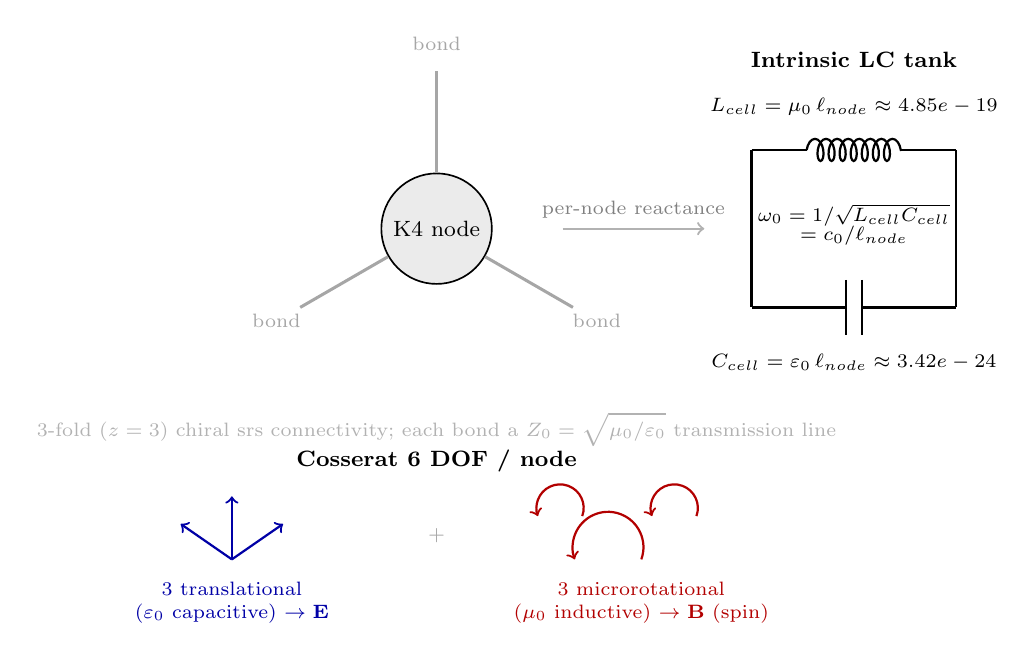
\begin{tikzpicture}[scale=1.0, transform shape,
    dofE/.style={->, thick, blue!65!black},
    dofB/.style={->, thick, red!70!black},
    every node/.style={font=\footnotesize}]

    % --- central node ---
    \node[circle, draw, fill=black!8, minimum size=1.25cm, line width=0.6pt] (node) at (0,0) {K4 node};

    % --- 3-fold (z=3) chiral srs nearest-neighbour bond stubs (trivalent Laves connectivity) ---
    % z=3-diamond -> z=3-chiral-srs restoration (2026-07-04; discharges the af1 figure debt
    % logged in research/2026-07-03_axiom1-dof-restoration_note.md). srs/Sunada-K4 is DEGREE-3;
    % the former 4-stub tetrahedral geometry depicted the doubly-ratified-against z=4 diamond.
    \foreach \ang/\lab in {90/{}, 210/{}, 330/{}} {
        \draw[line width=1.1pt, gray!70] (node) -- (\ang:2.0);
        \node[gray!70, font=\scriptsize] at (\ang:2.35) {bond};
    }
    \node[gray!60, font=\scriptsize, align=center] at (0,-2.55)
        {3-fold ($z=3$) chiral srs connectivity; each bond a $Z_0=\sqrt{\mu_0/\varepsilon_0}$ transmission line};

    % --- intrinsic LC tank (drawn to the right as the node's internal reactance) ---
    \begin{scope}[shift={(5.3,0)}]
        \node[font=\footnotesize\bfseries] at (0,2.15) {Intrinsic LC tank};
        % inductor (coil) top branch
        \draw[line width=0.8pt] (-1.3,1.0) -- (-0.6,1.0);
        \draw[line width=0.8pt, decorate, decoration={coil, aspect=0.5, segment length=4pt, amplitude=4pt}]
              (-0.6,1.0) -- (0.6,1.0);
        \draw[line width=0.8pt] (0.6,1.0) -- (1.3,1.0);
        \node[align=center, font=\scriptsize] at (0,1.55) {$L_{cell}=\mu_0\,\ell_{node}\approx\SI{4.85e-19}{\henry}$};
        % capacitor bottom branch
        \draw[line width=0.8pt] (-1.3,-1.0) -- (-0.1,-1.0);
        \draw[line width=0.8pt] (-0.1,-0.65) -- (-0.1,-1.35);
        \draw[line width=0.8pt] (0.1,-0.65) -- (0.1,-1.35);
        \draw[line width=0.8pt] (0.1,-1.0) -- (1.3,-1.0);
        \node[align=center, font=\scriptsize] at (0,-1.7) {$C_{cell}=\varepsilon_0\,\ell_{node}\approx\SI{3.42e-24}{\farad}$};
        % side wires closing the loop
        \draw[line width=0.8pt] (-1.3,1.0) -- (-1.3,-1.0);
        \draw[line width=0.8pt] (1.3,1.0) -- (1.3,-1.0);
        \node[align=center, font=\scriptsize] at (0,0.05)
            {$\omega_0 = 1/\sqrt{L_{cell}C_{cell}}$\\[-1pt] $= c_0/\ell_{node}$};
    \end{scope}
    \draw[->, gray!60, line width=0.8pt] (1.6,0) -- (3.4,0)
        node[midway, above, font=\scriptsize, gray] {per-node reactance};

    % --- the Cosserat 6-DOF split (below) ---
    \begin{scope}[shift={(0,-4.2)}]
        \node[font=\footnotesize\bfseries] at (0,1.25) {Cosserat 6 DOF / node};
        % 3 translational -> E
        \draw[dofE] (-2.6,0) -- (-2.6,0.8);
        \draw[dofE] (-2.6,0) -- (-1.95,0.45);
        \draw[dofE] (-2.6,0) -- (-3.25,0.45);
        \node[blue!65!black, align=center, font=\scriptsize] at (-2.6,-0.55)
            {3 translational\\($\varepsilon_0$ capacitive) $\to \mathbf{E}$};
        % 3 microrotational -> B
        \draw[dofB] (2.6,0) arc (-20:200:0.45);
        \draw[dofB] (1.85,0.55) arc (-20:200:0.30);
        \draw[dofB] (3.3,0.55) arc (-20:200:0.30);
        \node[red!70!black, align=center, font=\scriptsize] at (2.6,-0.55)
            {3 microrotational\\($\mu_0$ inductive) $\to \mathbf{B}$ (spin)};
        \node[gray!70, font=\scriptsize] at (0,0.3) {$+$};
    \end{scope}

\end{tikzpicture}
\caption{K4 node anatomy. Each node of the chiral Laves K4 Cosserat lattice carries one intrinsic electromagnetic LC tank ($L_{cell}=\mu_0\ell_{node}\approx\SI{4.85e-19}{\henry}$, $C_{cell}=\varepsilon_0\ell_{node}\approx\SI{3.42e-24}{\farad}$; \kbleaf{src/ave/core/constants.py} \texttt{L\_CELL}, \texttt{C\_CELL}), resonating at $\omega_0=c_0/\ell_{node}=\sqrt{1/(L_{cell}C_{cell})}\approx\SI{7.76e20}{\radian\per\second}$ (\texttt{OMEGA\_C}), connects to its three nearest neighbours (3-fold $z=3$ chiral srs / Sunada-K4 / Laves connectivity) through $Z_0=\sqrt{\mu_0/\varepsilon_0}=\sqrt{L_{cell}/C_{cell}}\approx376.73\,\Omega$ bond transmission lines, and hosts six Cosserat degrees of freedom: three translational (capacitive $\varepsilon_0$, identified with $\mathbf{E}$) and three microrotational (inductive $\mu_0$, identified with $\mathbf{B}$; the substrate-native origin of intrinsic spin). Axioms~1 (substrate topology). Schematic; not driver-generated.}
\label{fig:vol9_node_anatomy}
\end{figure}


\begin{itemize}
    \item \textbf{Intrinsic LC oscillator at each node.} Each K4 node carries one electromagnetic LC tank with per-cell elements $L_{cell} = \mu_0\, \ell_{node}$ and $C_{cell} = \varepsilon_0\, \ell_{node}$. The substrate is an LC network at its smallest accessible scale (Axiom~1).
    \item \textbf{Bond transmission lines.} Bonds connecting nearest-neighbour nodes carry distributed transmission-line topology (TLM), with characteristic impedance $Z_0 = \sqrt{\mu_0/\varepsilon_0} \approx \qty{376.73}{\ohm}$ scale-invariant in the lattice pitch.
    \item \textbf{Cosserat micropolar 6 DOF per node.} Each node carries six intrinsic degrees of freedom: three \textbf{translational} (capacitive coupling $\varepsilon_0$, identified with the electric field $\mathbf{E}$) and three \textbf{microrotational} (inductive coupling $\mu_0$, identified with the magnetic field $\mathbf{B}$). The Cosserat microrotational DOF is the substrate-native origin of intrinsic spin.
    \item \textbf{Universal saturation kernel.} The Axiom~4 quarter-arc kernel $S(A) = \sqrt{1 - (A/A_{yield})^2}$ governs every cross-scale saturation event. Dielectric specialization at atomic / bench scale: $C_{eff} = C_0/S$, $\varepsilon_{eff} = \varepsilon_0 S$, $\mu_{eff} = \mu_0 S$. The same kernel governs Schwinger pair production, gravitational time dilation (via $c_{shear} = c_0 \sqrt{S}$), and every topological-reorganization event documented in Vol~0 backmatter.
    \item \textbf{$\Gamma$ boundary semantics (three-channel, one external + two confined).} Substrate boundaries carry channel-subscripted reflection coefficients $\Gamma_{\mathrm{EM}}$, $\Gamma_{\mathrm{shear}}$, $\Gamma_{\mathrm{bulk}}$ with impedances $Z_{\mathrm{EM}} \equiv Z_0$, $Z_{\mathrm{shear}} = \rho c_{\mathrm{shear}}$, $Z_{\mathrm{bulk}} = \rho c_{\mathrm{bulk}}$ (three-impedance law; KB \kbleaf{ave-kb/vol9/ch4-dc-electrical-characteristics/three-channel-impedances.md}). Axiom~3 minimizes $|\Gamma|^2$ per channel. The three channels are \emph{asymmetric in port role}: the EM channel is the substrate's \textbf{sole external port} --- it is matched, $\Gamma_{\mathrm{EM}} = 0$, $Z_{\mathrm{EM}} \equiv Z_0$ everywhere, and is how a bound interior couples to the far field (a radiative port, not a hair-sector). The two \emph{mechanical} channels (shear $=$ charge, bulk $=$ mass) are \textbf{confined}: $\Gamma_{\mathrm{shear}}, \Gamma_{\mathrm{bulk}} \to -1$ at the saturated cage wall ($Z = Z_0\sqrt{S} \to 0$), short-circuit boundaries that trap the soliton rather than radiate it. One external port plus two confined mechanical ports is the load-bearing node topology (KB \kbleaf{ave-kb/vol9/ch3-pin-port-configuration/device-circuit-models.md} \S6.1). Device equivalent circuits: same leaf; PDF figures Ch.~\ref{ch:vol9_pin_port_configuration}~\S\ref{sec:vol9_device_circuit_models}.
    \item \textbf{Saturable yield and breakdown thresholds.} The substrate has two distinct dielectric thresholds (Vol~4; \kbleaf{ave-kb/vol4/circuit-theory/ch2-topological-thrust-mechanics/dielectric-yield-thresholds.md}): the macroscopic nonlinear-onset $V_{yield} = \sqrt{\alpha}\, V_{snap} \approx 43.65\,\text{kV}$ and the absolute topological node-destruction limit $V_{snap} = m_e c^2/e \approx 511\,\text{kV}$. Engineering practice operates well below $V_{yield}$ in linear-regime devices; AVE substrate-physics describes the saturating, breakdown, and rupture regimes via the four-regime map (Vol~1 Ch.~\ref{ch:regime_map}).
    \item \textbf{Topological transduction.} The Topological Conversion Constant $\xi_{topo} = e/\ell_{node} \approx \qty{4.149e-7}{\coulomb\per\metre}$ is the substrate-native bridge between electrical and mechanical observables (Axiom~2). Every spec in this datasheet that crosses the EE/mechanical boundary carries $\xi_{topo}$ as the canonical mapping.
\end{itemize}

\section{Epistemic Position}
\label{sec:vol9_epistemic_position}

This datasheet adopts the same epistemic stance as a manufacturer's component datasheet for a natural material (e.g., copper at the OFE grade, single-crystal silicon, or fused quartz): the material is natural, its properties are empirically characterized, and its parameters are derived from the material's microscopic structure where derivation is possible. The substrate documented here is the natural vacuum. Engineering characterization is the empirical-measurement side; AVE substrate-physics is the first-principles-derivation side. The datasheet documents both columns.

\subsection{FORM-deriving / VALUE-importing}
\label{subsec:vol9_form_vs_value}

The derivation column above splits one level deeper, and the split is load-bearing for how every spec in this datasheet should be read. The geometry and topology of the chiral K4 Cosserat substrate \textbf{FORCE the dimensionless FORMS} --- the structure: the integer/geometric skeleton of a result (the $/7$ PPN couplings, $\sin^2\theta_W = 2/9$, $\nu_{vac} = 2/7$, $g_* = 7^3/4$, exact-quantized charge, the spin-statistics phase). The \textbf{dimensionful VALUES of the handful of calibration constants the substrate is \emph{fed}} are calibration inputs it does not independently select. In the framework's standing vocabulary, a forced form is a \emph{chord} and an imported value is an \emph{echo} (canonical leaf \kbleaf{ave-kb/common/form-deriving-value-importing.md}; the canonical chord / echo / mixed definitions at \kbleaf{ave-kb/common/vocabulary-register.md}).

The calibration set is three dimensionful constants $\{m_e, \alpha, G\}$ plus the four axioms; every other quantity follows as a geometric ratio of $\ell_{node}$. Per the settled per-constant accounting: $\alpha$ is an \textbf{echo} (its decomposition FORM $4\pi^3 + \pi^2 + \pi$ is forced; the exact \emph{value} rests on the named identification $R\cdot r = 1/4$ the substrate does not independently select); $G$ is \textbf{mixed} (the Achromatic-Lens $/7$ projection FORM is derived, the $\xi$ value-fitted to CODATA $G$); $K = 2G$ ($\nu_{vac} = 2/7$) is \textbf{GR-imported} for its value; $E_{yield}$ is \textbf{mixed} (the \emph{existence} of a yield field is an AVE-distinct chord, its $\sqrt{\alpha}$ \emph{value} rides the $\alpha$-echo); $m_e/\ell_{node}$ is \textbf{definitional} (the Axiom-1 calibration anchor). This is not a deflation: forcing the exact dimensionless skeleton from topology is a strong falsifiable claim, untouched by the value-import finding --- and the FORM-deriving half applies to all five constants.

The testing consequence is recorded in Ch.~\ref{ch:vol9_falsification_tests}: because every dimensionful magnitude is an echo by construction, an AVE-distinct \emph{discriminating} prediction lives only in (a) FORM-EXISTENCE divergences (a structure the SM vacuum lacks --- saturation, the longitudinal scalar, native birefringence) and (b) FORCED DIMENSIONLESS RATIOS that do not dissolve into $\alpha$, $G$, or $m_e$. The Ch.~\ref{ch:vol9_falsification_tests} forward-prediction register classifies each chapter's predictions on this axis.

Per the EE-as-substrate-native META framework (canonical leaf \kbleaf{ave-kb/common/translation-tables/translation-circuit.md}), electrical engineering vocabulary is the closest-to-canonical substrate-native language: the substrate is an LC network at minimal degrees of freedom, and EE was developed by humans empirically interrogating that substrate at its smallest accessible scale (electron dynamics in conductors, dipole interactions in dielectrics, LC resonant circuits, transmission lines, semiconductor breakdown). Vol~9 datasheet vocabulary is therefore EE-primary throughout; other classical frameworks (atomic physics, chemistry, statistical mechanics, fluid dynamics, GR, QFT) layer additional degrees of freedom on top of the EE base and are invoked only where they capture content the EE projection does not (geometric, topological, axiom-selection content; see Vol~9 Ch.~13 application examples).

\section{How to Use This Datasheet}
\label{sec:vol9_how_to_use}

\subsection{Spec-table column convention}

Each parameter spec table in subsequent chapters carries the following columns:

\begin{itemize}
    \item \textbf{Symbol} --- canonical AVE symbol (per CLAUDE.md INVARIANT-S2 axiom statements and Vol~1 notation).
    \item \textbf{Typical} --- canonical value under standard operating conditions ($T = T_{CMB}$ unless noted; cold-lattice limit $S(0) = 1$).
    \item \textbf{Min / Max} --- characterized range, where applicable. Many substrate primitives are fixed (no range); for these, Min / Max columns are omitted or marked ``---''.
    \item \textbf{Units} --- SI units, except where dimensionless or topological.
    \item \textbf{Conditions} --- operating-point conditions ($A_0$, $T$, boundary class SYM/ASYM, regime I--IV).
    \item \textbf{Canonical Source} --- pointer to the derivation leaf in Vol~1--6 (KB leaf path + claim ID where applicable).
\end{itemize}

\subsection{Cross-reference structure}

Vol~9 is a synthesis volume; no chapter contains a primary derivation. Every spec table points to the canonical leaf in Vols~1--6 where the substrate-physics derivation lives. Cross-references use \texttt{xr-hyper} to resolve chapter and section numbers across the volume set. To resolve all references, build the dependent volumes first (\texttt{make vol1 vol3 vol4 vol0}) then \texttt{make vol9}.

\subsection{Falsification integration}

Engineering datasheets typically end with electrical characteristics, mechanical characteristics, and application examples. This datasheet adds \textbf{Ch.~15 Falsification Tests}: every load-bearing substrate-physics claim is tied to at least one bench-falsifiable experiment (PONDER-05 dielectric saturation, HOPF-01 chiral antenna, Sagnac-RLVE, right-handed-neutrino kill-switch, quasar $\alpha$-variation, etc.). The substrate is the natural medium; the framework that derives its behaviour is falsifiable.

\section{Chapter Sequence and Canonical Source Map}
\label{sec:vol9_chapter_map}

\begin{table}[htbp]
\centering
\begin{tabular}{p{0.05\linewidth} p{0.35\linewidth} p{0.50\linewidth}}
\toprule
\textbf{Ch} & \textbf{Topic} & \textbf{Primary canonical source(s)} \\
\midrule
2  & Absolute Maximum Ratings           & Vol~1 + Vol~4 canonical constants; four-regimes Regime IV \\
3  & Pin / Port Configuration           & Vol~1 universal operators (Op17, Op21); $\Gamma$ boundary classes; device circuit models (\texttt{AVE\_VACUUM\_CELL}, electron TIR tank) \\
4  & DC Electrical Characteristics      & \kbleaf{src/ave/core/constants.py}; natural-units cheatsheet \\
5  & AC Electrical Characteristics      & Vol~1 Ch.~5 universal spatial tension; Op14 / Op16 \\
6  & Temperature Characteristics        & Cosserat-Curie $\delta_{strain}$ at $T_{CMB}$; translation-circuit \S 9 \\
7  & Saturation Characteristics         & Axiom~4 kernel; Vol~0 backmatter Ch.~7 universal saturation kernel \\
8  & Breakdown Characteristics          & Schwinger pair production; Miller avalanche; Regime~III \\
9  & Mechanical Characteristics         & Vol~3 $G_{vac}$, $K_{vac}$, Cosserat $\gamma_c$, $\nu_{vac} = 2/7$ \\
10 & Magnetic / Microrotational         & Cosserat flywheel L; rotation-sector mass-gap; weak-force $l_c$ \\
11 & Topological Characteristics        & $(2,3)$ knot uniqueness; $I4_1 32$ chiral space group \\
12 & Cosmological Characteristics       & $R_H/\ell_{node} \sim 10^{39}$ ($\approx 3.456\times10^{38}$); Machian $G$ (mixed); $u_0^* \approx 0.187$ (calibrated value, not substrate-selected) \\
13 & Application Examples               & Cross-references to canonical leaves \\
14 & Phase Diagrams                     & Four-regimes map; cosmic phase diagram \\
15 & Falsification Tests                & Vol~4 Ch.~11 experimental programme; kill-switch tests \\
16 & Cross-Volume Reference Index       & Auto-generated parameter $\to$ derivation map \\
17 & Engine Requirements                & Axiom-4 kernel gate; engine-acceptance suite (L0--L2); faithful-simulator spec \\
18 & Experimental Prints                & Topology laboratory exercises; bench falsification prints \\
19 & Calibration Parameter Justification & Consolidated calibration / reference conditions; master table (role + chord/echo/mixed) over $\{m_e, \alpha, G\}$ + SI / derived / cosmological-initial-data; \kbleaf{form-deriving-value-importing.md}; \kbleaf{interlock-register.md} \\
\bottomrule
\end{tabular}
\caption{Vol~9 chapter sequence with the primary canonical-leaf source(s) backing each datasheet chapter.}
\label{tab:vol9_chapter_map}
\end{table}

\noindent
Subsequent chapters populate the spec tables. Where a substrate primitive's derivation has not yet closed at substrate-axiom rigor (e.g., the substrate-statistical-mechanics derivation of $\eta_\varepsilon$ in $\delta_{strain}$ at $T_{CMB}$), the datasheet entry is marked with a footnote pointing to the open research question.
